%%%%%%%%%%%%%%%%%%%%%%%%%%%%%%%%%%%%%%%%%%%%%%%%%%%%%%%%%%%%%%%%%%% 
%                                                                 %
%                            CHAPTER TWO                         %
%                                                                 %
%%%%%%%%%%%%%%%%%%%%%%%%%%%%%%%%%%%%%%%%%%%%%%%%%%%%%%%%%%%%%%%%%%% 
 
\chapter{Homotopy-based Globalization}

\section{Homotopy-based Globalization}\label{sec:homotopy}
Homotopy methods are robust, numerically stable, and globally convergent methods
for solving nonlinear algebraic equations; see, for example,
\cite{allgower_georg_1993} and \cite{Watson_1989}.  Our interest in these
methods began as a means of globalizing difficult computational aerodynamics
problems~\cite{hicken:cfd2009, hicken:cfd2011b, Brown_2016}, but globally
convergent probability-one homotopy methods have also been successfully applied
to solve engineering optimization problems.  Watson~\cite{Watson_2001} reviewed
and developed the general convergence theory for nonlinear optimization
problems, including unconstrained, bound-constrained, linear and nonlinear
inequality constrained convex cases.  He also discussed the extension of the
theory to nonconvex problems, although the convergence theory for equality
constraints remains an open problem.  More recently, Huang
\etal~\cite{huang_2012pc} transformed a general nonlinear optimization with
equality and inequality into an inequality-only problem, and used a
predictor-corrector method to track the homotopy interior-point map using the
conjugate gradient method. While their method achieves global linear convergence
under the normal cone condition, it is limited to convex objective and
constraint functions.

\subsection{Example}

Conceptually, the idea of homotopy methods is easy to understand. To find the
solution of a difficult nonlinear equation, $F(q)=0$, a homotopy map is
constructed that connects the target problem to an easy-to-solve problem via a
parameter.  For example, a convex homotopy map $H : \mathbb{R}^N \times
\mathbb{R}^{N} \times [0,1) \rightarrow \mathbb{R}^N$ is given by
\begin{equation}\label{eq:homotopy}
H(q, q_0, \mu) = (1-\mu) F(q) + \mu G(q,q_0),\quad 0 \leq \mu \leq 1,
\end{equation}
where $\mu$ is the homotopy parameter, and $G : \mathbb{R}^N\times\mathbb{R}^{N}
\rightarrow \mathbb{R}^N$ is chosen such that $G(q,q_0)=0$ is easy to solve and
has the solution $q=q_0$.  Formally, a homotopy is a continuous map from the
interval $[0,1]$ into a function space.

We will use a simple, unconstrained optimization example to illustrate the
homotopy idea. Consider the problem
\begin{equation*}
\min_x  \quad  f(x) = x^4 - x^2.
\end{equation*}
The first-order optimality condition for this problem is given by (identifying
$q$ with $x$ here)
\begin{equation*}
F(x) = \nabla_x f(x) = 2x(2x^2 - 1) = 0.
\end{equation*}
It is easy to see that there are three stationary points; a local maximizer at
$x=0$ and two local/global minimizers at $x=\pm 1/\sqrt{2}$.  Newton's method
may converge to any of these stationary points depending on the initial guess
$x_0$, so we need some way to avoid the local maximizer at $x=0$.

Now, consider the simple problem $\min_x \; \frac{1}{2}(x - x_0)^2$, whose
first-order optimality is given by
\begin{equation*}
G(x,x_0) = x - x_0 = 0.
\end{equation*}
This has the obvious solution $x=x_0$.  We can take advantage of this simple
optimization problem by constructing a convex homotopy that combines $F(x)$ and
$G(x,x_0)$ as follows:
\begin{equation*}
  H(x, x_0, \mu) = (1-\mu) F(x) + \mu G(x, x_0) = (1 - \mu) 2x(2x^2 -1) + \mu (x
  - x_0).
\end{equation*}
Next, we trace out the set of solutions corresponding to $H(x,x_0,\mu)=0$ from
$\mu=1$ to $\mu=0$.  Starting at $\mu=1$ we have the solution $x=x_0$.  If we
change the value of $\mu$ slightly to $\mu = 1 - \Delta \mu$, then, for $\Delta
\mu$ sufficiently small and by continuity, $x_0$ should remain in the basin of
attraction for Newton's method applied to $H(x, x_0, 1-\Delta \mu)=0$.  The
solution at $\mu= 1 - \Delta \mu$ can then be used as an initial guess for the
next value of $\mu$, and so on, until we reach $\mu = 0$.  Example solution
paths for this process are illustrated in Figure~\ref{fig:zc} starting from
distinct $x_0$.  Notice that all paths converge to the local minimizers, even
those that begin near the maximizer $x=0$.

\begin{figure}[t]
  \centering
  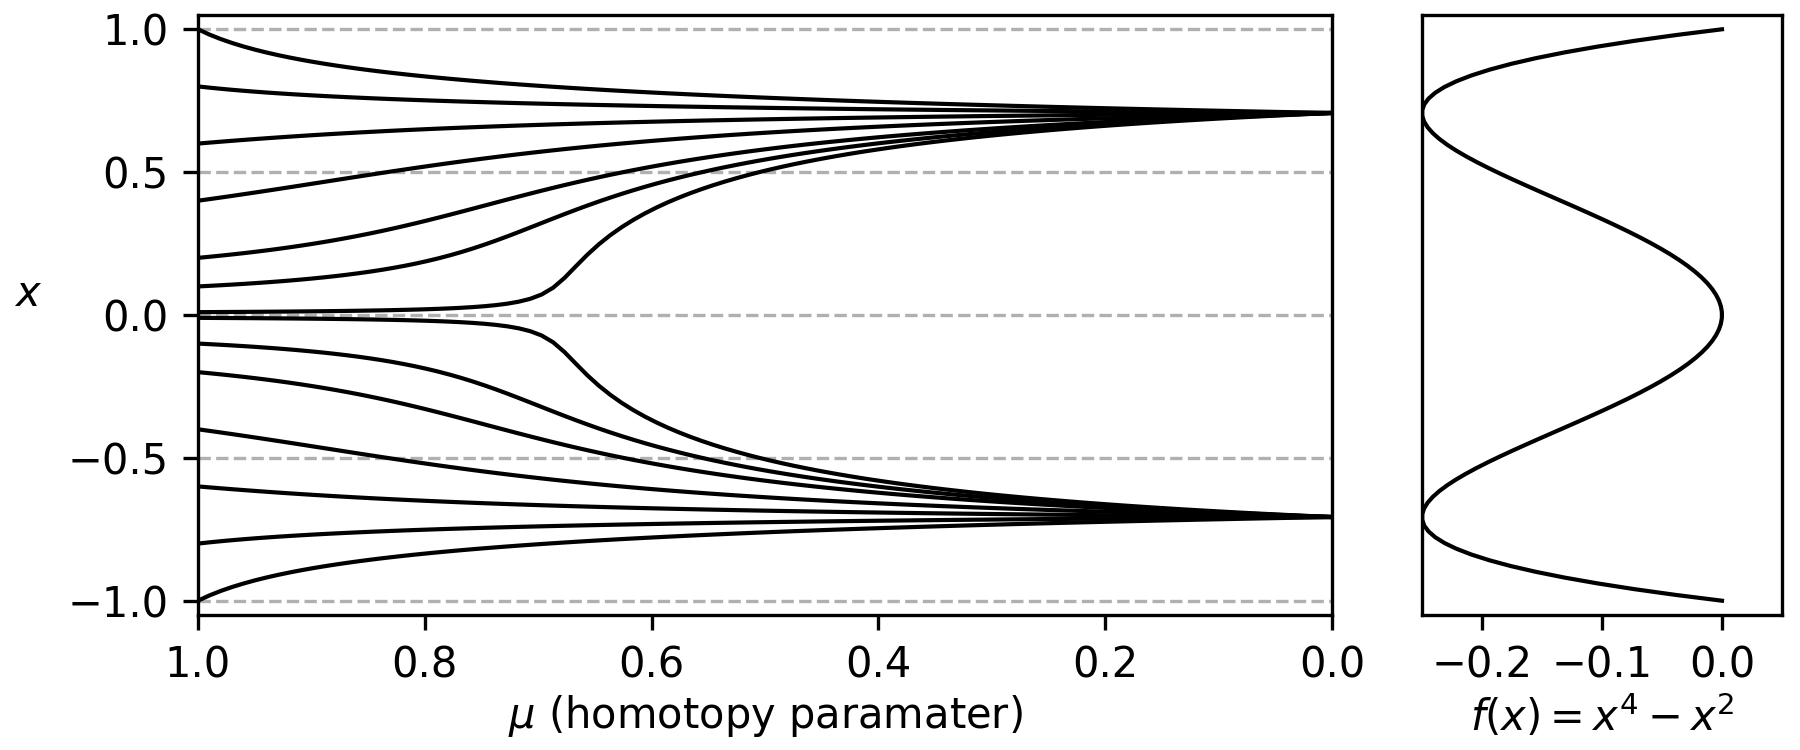
\includegraphics[width=\textwidth]{./figs/chap2/paths.png}
  \caption{Solution curves of $H(x,x_0,\mu) = 0$ (left side of figure) for
    different values of $x_0$.  The paths begin at $\mu=1$ and converge to the
    local minimizers at $\mu=0$.  The function to be minimized is plotted on the
    right-side of the figure.\label{fig:zc}}
\end{figure}

\subsection{Review of convergence theory for homotopy methods}

The path-following process described above, while intuitive, is not guaranteed
to succeed.  In particular, it is not clear that $\nabla_q H$ remains
non-singular along the path.  A poor choice of $G(q)$ may produce a level set
$H(q,q_0,\mu) = 0$ with an intersection, where $\nabla_q H$ is singluar and the path
bifurcates.  The Jacobian will also become rank deficient at so-called turning
points, where following the path from $\mu=1$ to $\mu=0$ requires $\mu$ to
increase at some point.  Finally, the path may diverge before reaching
$\mu=0$.

Many of the potential issues with the path-following approach can be avoided if
we place some conditions on the map $H$.  These conditions are described in the
theorem below, which has been adapted from~\cite{watson_2002} to the present
context.

\begin{theorem}\label{thm:homotopy}
  Assume the following conditions hold:
  \begin{itemize}
  \item $G : \mathbb{R}^{N} \times \mathbb{R}^{N} \rightarrow \mathbb{R}^{N}$ is
    a $C^2$ map, and $q=q_0$ is the unique solution to $G(q,q_0) = 0$;    
  \item $F :\mathbb{R}^{N} \rightarrow \mathbb{R}^{N}$, the first-order
    optimality residual given by \eqref{eq:opt00x}, is a $C^2$ map;
  \item For the homotopy map $H$ defined by \eqref{eq:homotopy}, the Jacobian
    $\nabla H \equiv \begin{bmatrix} \nabla_q H & \nabla_{q_0} H & \nabla_\mu
    H \end{bmatrix}$ is full-rank on the zero set $X \equiv \{(q,q_0,\mu) |
    H(q,q_0,\mu) = 0 \}$.
  \end{itemize}
  Then, for almost all $q_0 \in \mathbb{R}^{N}$, there exists a zero curve of
  $H$ starting from $q=q_0$ at $\mu=1$ along which the Jacobian $\nabla H$ has
  full rank.  Furthermore, if the set $X$ is bounded, then the path includes a
  point $(q,q_0,\mu) = (q^*,q_0,0)$, \ie, where $H(q^{*},q_0,0) = F(q^{*}) = 0$.
  Finally, if the Jacobian $\nabla_q F$ is invertible at $q^{*}$, the path has
  finite arc length.
\end{theorem}

Theorem~\ref{thm:homotopy} is a powerful result.  It implies that, for almost
all choices of $q_0$, there exists a path from $q=q_0$ at $\mu=1$ to a point
$q=q^*$ at $\mu=0$ that satisfies $F(q^*) = 0$, and along this path the Jacobian
is full-rank.  The phrase \emph{``almost all choices of $q_0$''} means that the
set of points for which there is no path has measure zero.

The drawback of Theorem~\ref{thm:homotopy} is that its assumptions, with the
exception of the first, are difficult to guarantee or verify in
practice\footnote{The first condition requires $G$ to be sufficiently smooth and
  have $q_0$ as its only solution; as we show in Section~\ref{sec:map}, it is
  straightforward to construct such a map.}.  The second condition, which cannot
be relaxed~\cite{watson_2002}, implies that the objective and constraints are
$C^3$.  While this level of smoothness exists for many engineering problems, it
is certainly not true in general.  The third assumption means that $H$ is
\emph{transversal to zero} for each choice of $q_0$, which can be verified for
simple problems, but may be difficult to determine for complex engineering
design problems.  Finally, as Watson points out in~\cite{watson_2002}, the
assumptions on the boundedness of the path and the invertibility of $\nabla_q F$
at $q^{*}$ are the most difficult to verify, since, taken together with the
other conditions, they imply the exsistence of a solution to $F(q) = 0$.

Despite the potential difficulty of guaranteeing the assumptions of
Theorem~\ref{thm:homotopy}, the theorem hints at the robustness of the homotopy
approach, and this is corroborated by our experience.

\subsection{Homotopy map for constrained optimization}\label{sec:map}

For this work we use the convex homotopy defined by \eqref{eq:homotopy},
therefore we need only define $G(q,q_0)$.  Similar to the unconstrained case, we
could use a map of the form
\begin{equation*}
  G(q,q_0) = q - q_0,
\end{equation*}
where $q_0 = \begin{bmatrix} x_0^T & s_0^T & \lambda_{h0}^T &  \lambda_{g0}^T \end{bmatrix}^T$.  However, this map produces a
positive-definite (diagonal) Jacobian $\nabla_q G$, which would be inconsistent
with the inertia of the Jacobian $\nabla_q F$ at a local solution to
\eqref{eq:opt00x}~\cite{Nocedal2006NO}.  Instead, we adopt the map
\begin{equation*}
  G(q,q_0) \equiv \begin{bmatrix}
    (x - x_0)^T &
    (s - s_0)^T &
    -\lambda_h^T & 
    -\lambda_g^T
  \end{bmatrix}^T, 
\end{equation*}
for which $q_0 = \begin{bmatrix} x_0^T & s_0^T & 0^T & 0^T \end{bmatrix}$.
We note that $G(q,q_0)$ satisfies the requirements of
Theorem~\ref{thm:homotopy}. 

For future reference, we restate the homotopy map that we use for solving the
first-order necessary conditions in this work:
\begin{equation}\label{eq:homo0}
    H(q, q_0, \mu) = (1-\mu)
    \begin{bmatrix}
      \nabla_x f(x) +   \lambda_h^T \nabla_x h(x)  +  \lambda_g^T \nabla_x g(x) \\
      -\mat{S}\mat{\Lambda_g} e \\
      h(x) \\
      g(x) - s 
    \end{bmatrix}
    + \mu
    \begin{bmatrix}
      x - x_0 \\
      s - s_0 \\
      -\lambda_h \\
      -\lambda_g
    \end{bmatrix}.
\end{equation}

\begin{remark}
  The homotopy map \eqref{eq:homo0} can be used to identify stationary points of
  $F(q)$, but it cannot, on its own, ensure that $s_i \geq 0$ and $\lambda_{i}
  \leq 0$.  We use safeguards to ensure the correct signs for the slacks and
  inequality multipliers; see Section~\ref{sec:fraction}.
\end{remark}

The homotopy map \eqref{eq:homo0} is a favorable in the context of optimization
for several reasons.  First, the term $\mu(x-x_0)$ helps to address nonconvexity
by adding a positive diagonal matrix to the Lagrangian Hessian during the early
stages of convergence.  Furthermore, the term $\mu(s - s_0) with s_0 > 0$ generates a path
that remains feasible with respect to the slack boundaries $s>0$.  Finally, the
term $-\mu\lambda_{h} \text{and}  -\mu\lambda_{g}$ improves the conditioning of the
KKT matrix; even when the constraint Jacobian is rank deficient the homotopy map
will remain invertible.

\section{Predictor-Corrector Path-following Algorithm}\label{sec:pc}
The theory presented in Section~\ref{sec:homotopy} tells us when a path exists
between $q_0$ and a solution to $F(q)$, but it does not tell us how to traverse
such a path in an efficient manner.  In this section we describe the modified
predictor-corrector algorithm~\cite{allgower_georg_1993} used to trace the
zero-curve of the homotopy map.

\subsection{Overview}

Figure \ref{fig:pc} illustrates the predictor and corrector phases at iteration
$k$.  The iteration begins by computing an inexact tangent to the path,
$q_{k+1}'$, and using this tangent to predict the next point on the path.
Subsequently, the homotopy parameter $\mu$ is fixed and a correction is found
that gives an inexact root of the homotopy.  This cycle is repeated until $\mu <
\epsilon_\mu$, where $\epsilon_\mu > 0$ is a specificed tolerance.  Once $\mu$ is
sufficiently close to zero an approximate solution of the primal-dual system is
recovered.

\begin{remark}
  We use a default value of $\epsilon_\mu = 10^{-9}$ in our algorithm, which we
  have found works well for most problems; however, for difficult problems, \eg,
  with rank-deficient constraint Jacobians, it may be necessary to use larger
  thresholds.  For example, we use $\epsilon_\mu = 10^{-6}$ in the structural
  optimization problem presented later.
\end{remark}

\begin{figure}[tbp]
  \centering
  \subfloat[exact solves \label{fig:exact_pc}]{
    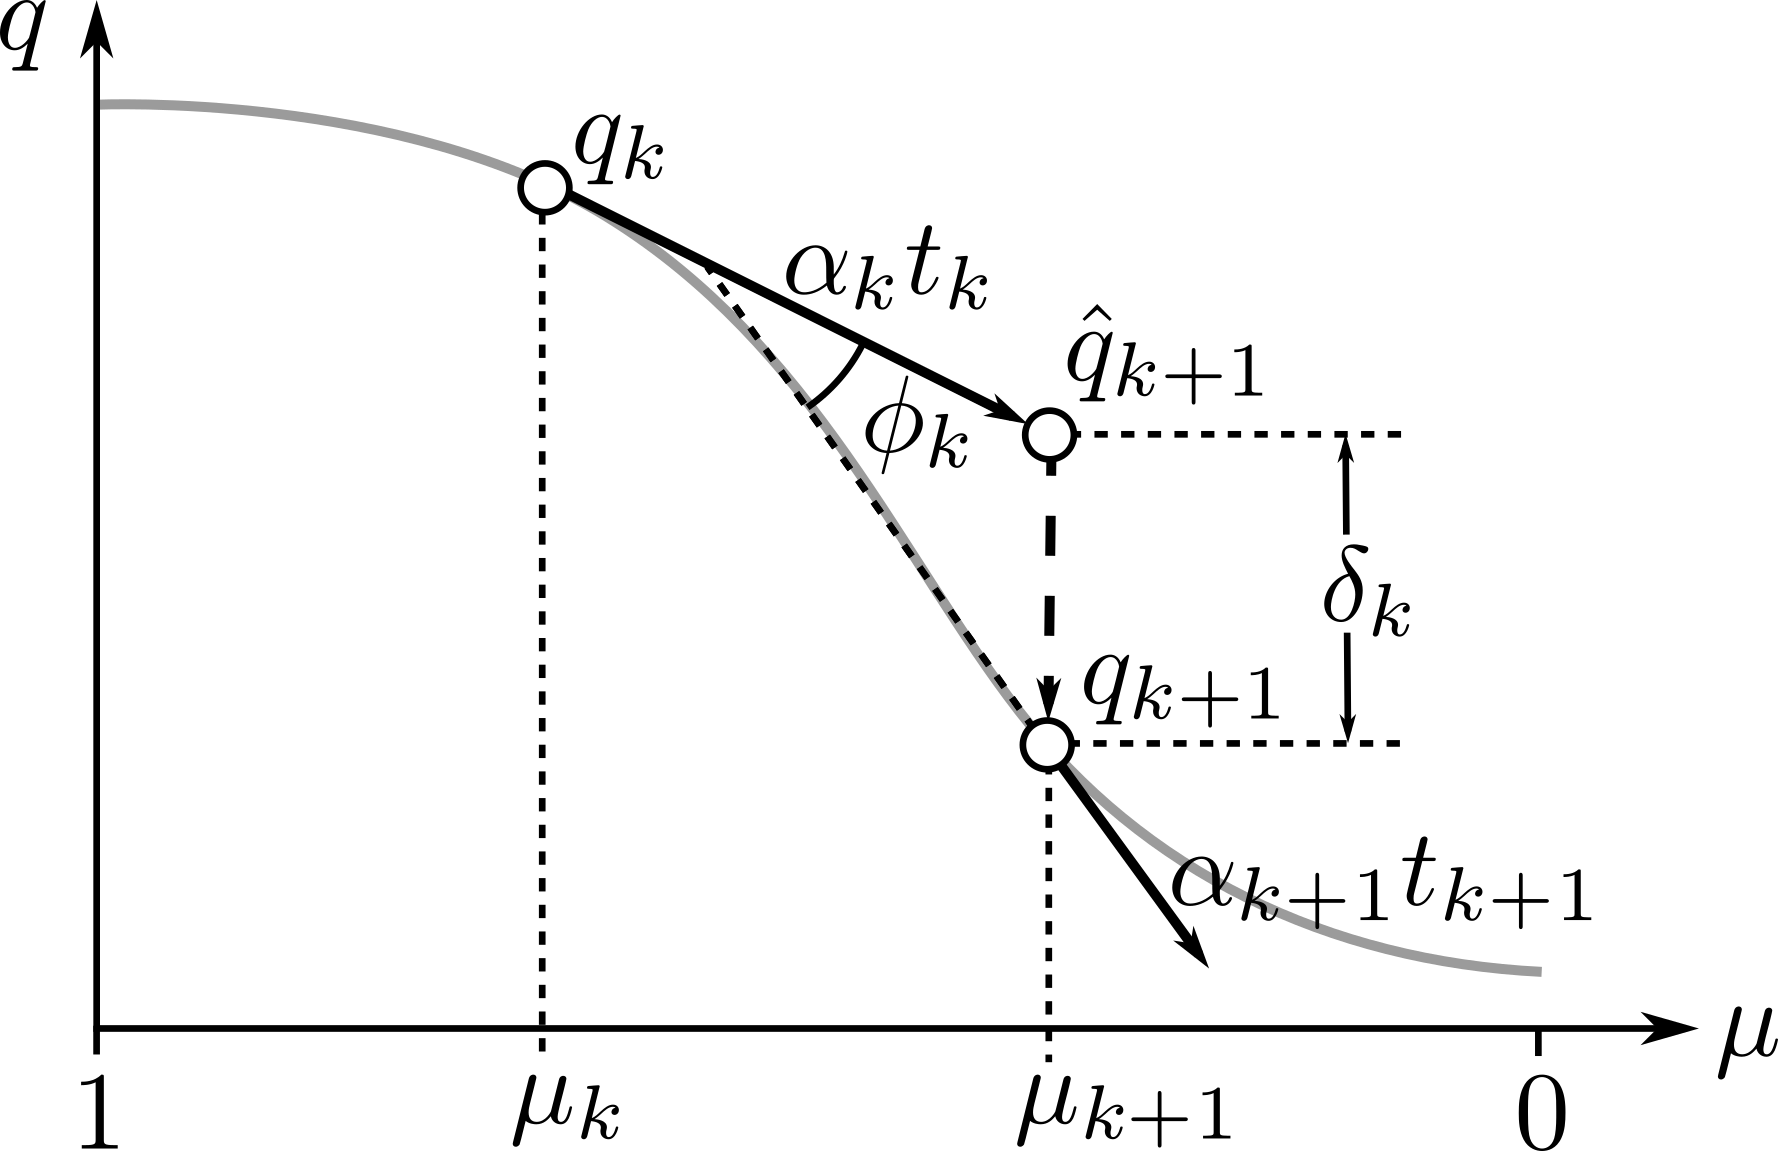
\includegraphics[width=0.4\linewidth]{figs/chap2/exact_pc.png} }
  \hspace{3em}
  \subfloat[inexact solves\label{fig:inexact_pc}]{
  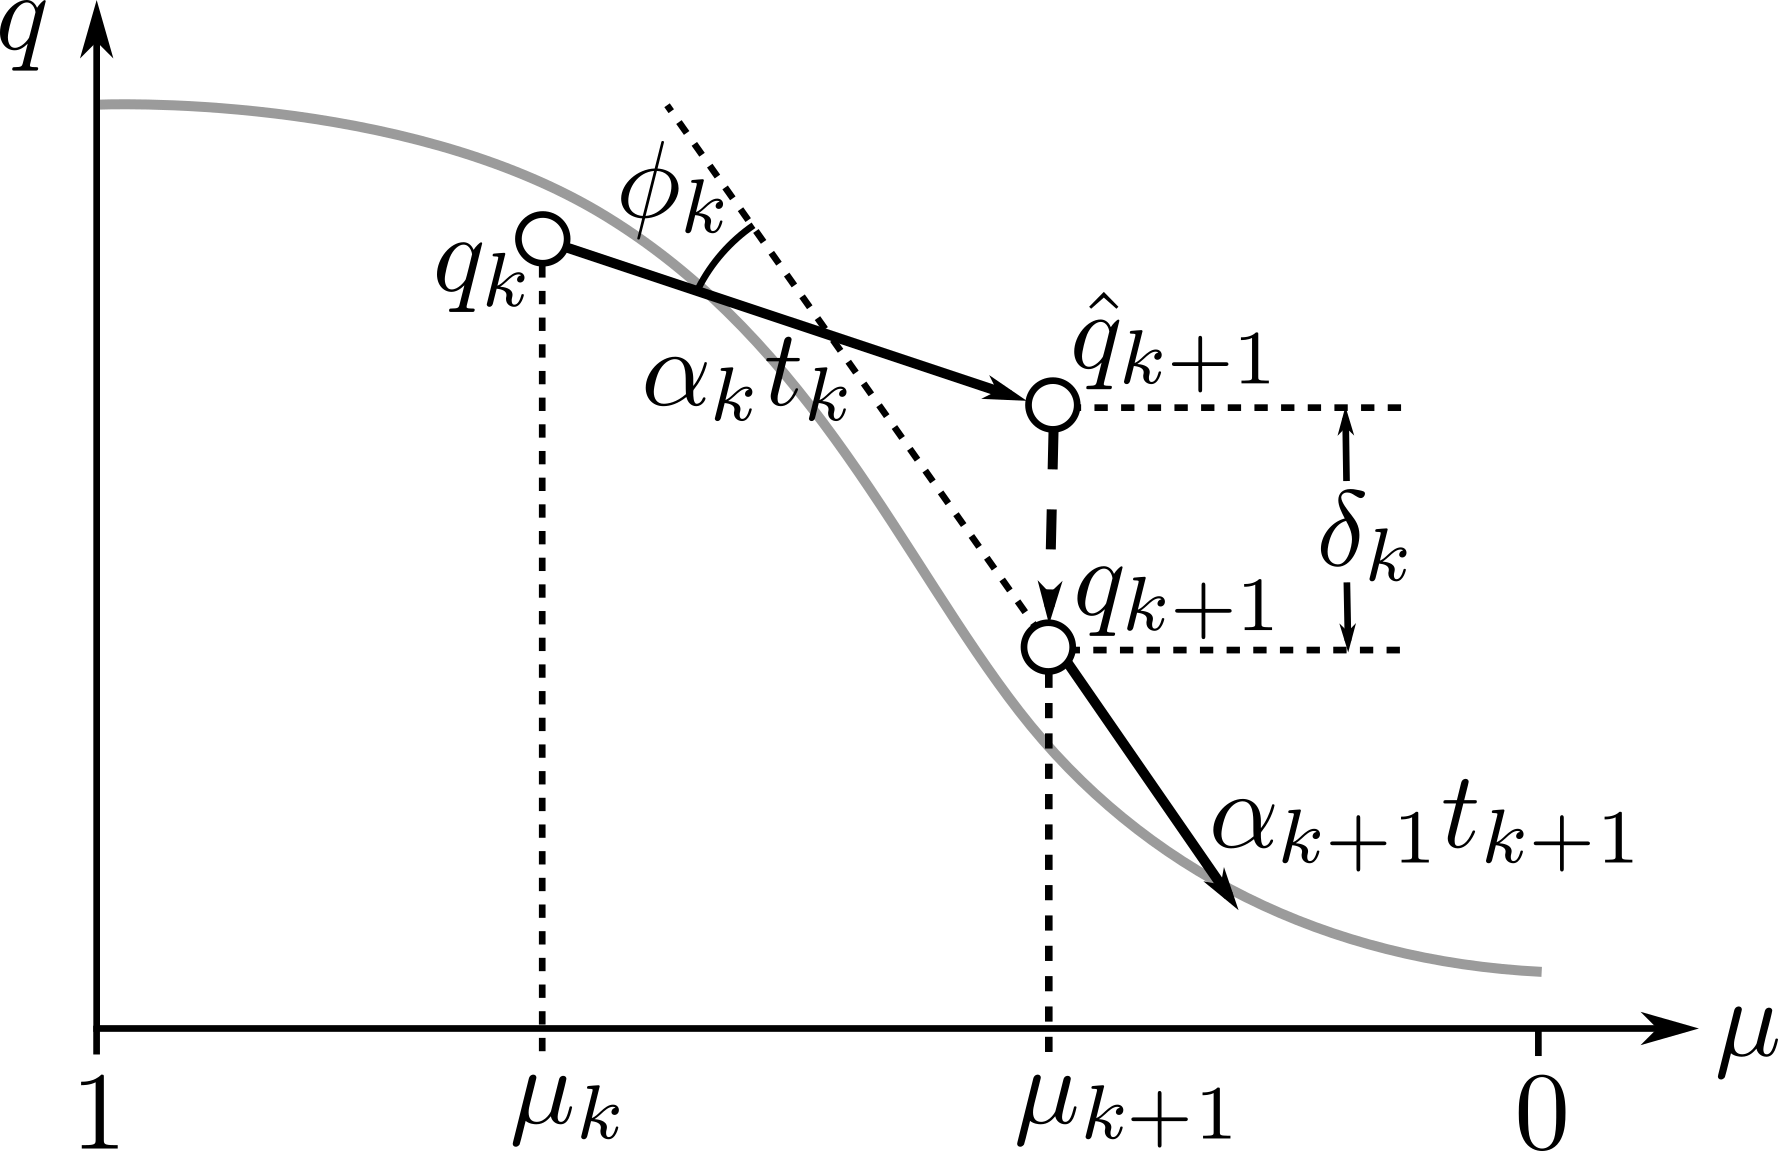
\includegraphics[width=0.4\linewidth]{figs/chap2/inexact_pc.png}
  }
 \caption{ Figure~\ref{fig:exact_pc} illustrates the predictor-corrector algorithm in the case that exact solves are used, while Figure~\ref{fig:inexact_pc} depicts the situation when inexact solves are used. \label{fig:pc}}   
\end{figure}


\begin{description}

  \item[Predictor:] During the predictor phase we first need to compute an
    approximate tangent direction $q' = dq/d\mu$, which is defined by taking the
    total derivative of $H(q,q_0,\mu) = 0$ with respect to $\mu$, \ie the
    implicit function theorem:
    \begin{equation}
      \left(\nabla_q H\right)_{k} q_{k}' = -\nabla_\mu H_{k} = F(q_k)  - G(q_k,q_0)
      \label{eq:predictorx}
    \end{equation}
    where $\nabla_q H$ and $\nabla_\mu H$ are evaluated at $q_k$, the previous
    homotopy iterate.  In practice, we solve \eqref{eq:predictorx} inexactly
    using a preconditioned Krylov iterative method.  That is, we find a $q_{k}'$
    that satisfies
    \begin{equation*}
      \lVert \left(\nabla_q H\right)_{k} q_{k}' - F(q) + G(q,q_0) \rVert
      \leq \tau \lVert F(q_k)  - G(q_k,q_0) \rVert,
    \end{equation*}
    where $\tau \in [0,1)$ is the desired relative tolerance.  Further details
      on the inexact solution of \eqref{eq:predictorx} are provided in
      Chapter~\ref{chap:linsys}.
    
    After (inexactly) solving \eqref{eq:predictorx} for $q_{k}'$, the predictor
    step is given by
    \begin{equation*}\label{eq:pred}
      \begin{bmatrix}
        \hat{q}_{k+1} \\ \mu_{k+1} 
      \end{bmatrix} 
      = \begin{bmatrix}
        q_k \\ \mu_k 
      \end{bmatrix}      
      + \alpha_{k} t_{k},
    \end{equation*}
    where $\alpha_{k}$ is the step length taken along the tangent direction at
    iteration $k$ (see Section~\ref{sec:step}), and $t_k$ is the normalized
    tangent given by
    \begin{equation*}
      t_{k} \equiv \frac{1}{\sqrt{\|q_{k}'\|^2 + 1}} \begin{bmatrix} -q_k'
        \\ -1 \end{bmatrix}.
    \end{equation*}
    Note that the negative signs in the definition of $t_k$ account for
    decreasing $\mu$ as the path moves from $\mu=1$ to $\mu <
\epsilon_\mu$.

  \item[Corrector:] In the corrector phase, we fix the homotopy parameter
    at $\mu=\mu_{k+1}$ based on the predictor, and use a Newton-Krylov method to
    inexactly solve $H(q_{k+1},q_0,\mu_{k+1}) = 0$.  This has the effect of
    ``correcting'' $\hat{q}_{k+1}$ to be closer to the path.  More precisely,
    we seek $q_{k+1}$ that reduces the relative residual below some tolerance:
    \begin{equation}\label{eq:cornt}
      \lVert H(q_{k+1},q_0,\mu_{k+1}) \rVert \leq
      \epsilon_k \lVert H(\hat{q}_{k+1},q_0,\mu_{k+1}) \rVert.
    \end{equation}
    A loose relative tolerance of $\epsilon_k \in [0.1,0.5]$ is used for
    homotopy parameter values $\mu > 0$ to avoid oversolving the corrector step.
    Once the algorithm reaches $\mu = 0$, the tolerance is tightened to the
    user-specified value for the first-order necessary conditions.
    
    At each Newton subiteration within the corrector, we must solve a linear
    system of the form
    \begin{equation}\label{eq:cor}
      \left(\nabla_q H \right)_{k+1} \Delta q_{k+1} = -H,
    \end{equation}
    for $\Delta q_{k+1}$, where $(\nabla_q H)_{k+1}$ and $H_{k+1}$ are evaluated
    at $\mu_{k+1}$ and the current estimate for $q_{k+1}$.  The Jacobian,
    $\nabla_q H$, that appears in \eqref{eq:cor} also appears in
    \eqref{eq:predictorx} during the predictor phase; again, further details
    regarding the solution of the linear systems that involve $\nabla_q H$ are
    provided in Chapter~\ref{chap:linsys}.

\end{description}

\begin{remark}
  The above predictor-corrector approach is a classical embedding
  method~\cite{allgower_georg_1993}, since the solution path is assumed to be
  parameterized by $\mu$; that is, the path has the form $(q(\mu),\mu)$.  This
  type of method cannot handle folds, or turning points, where the path reverses
  direction with respect to $\mu$ and the Jacobian $\nabla_q H$ becomes
  singular.  Problems for which such turning points arise can be handled using
  more advanced predictor-corrector algorithms; see, for
  example,~\cite{walker:1999}.
\end{remark}

\subsection{Implementation details}

\subsubsection{Adaptive step-size control}\label{sec:step}

The step length $\alpha$ along the tangent direction is calculated using the
asymptotic expansion method \cite{allgower3}, which we briefly review here.

At the first iteration of the predictor-corrector algorithm when $\mu=1$, a
conservative step length is used, \eg, $\alpha_0 = 0.05$.  Subsquent step
lengths are then determined adaptively using a scaling factor and a couple
safeguards on the maximum step size:
\begin{equation*}
  \alpha_{k} = \min\left( \sqrt{\|q_{k}'\|^2 + 1}\Delta \mu_{\max}, \alpha_{\max}, \alpha_{k-1}/\zeta_{k} \right),
\end{equation*}
where $\Delta \mu_{\max}$ is the maximum allowable change in $\mu$,
$\alpha_{\max}$ is allowable step size permitted by the fraction-to-the-boundary
rule (see Section~\ref{sec:fraction}), and the scaling factor is given by
\begin{equation*}
  \zeta_{k} \equiv \max\left( \sqrt{\delta_k/\delta_{\text{targ}}}, \phi_k / \phi_{\text{targ}} \right).
\end{equation*}

The scaling factor $\zeta_k$ is controlled by two quantities that measure how
nonlinear the path is, namely the previous corrector update size, and the angle
between successive tangents.  Referring to Figure~\ref{fig:pc}, the corrector
update size is the magnitude of the difference between the predictor step and
the corrector step:
\begin{equation}\label{eq:delta_k}
  \delta_k \equiv \| q_{k} - \hat{q}_{k} \|.
\end{equation}
A large value of $\delta_k$ indicates that the linear predictor does not
approximate the path well, so a smaller step size is warranted.  The angle
between the tangents is
\begin{equation}\label{eq:phi_k}
  \phi_k \equiv \arccos\left(t_{k+1}^T t_{k} \right).
\end{equation}
The angle $\phi_k$ is a measure of the curvature in the path, so a relatively
large value of $\phi_k$ also suggests that $\alpha_k$ should be reduced.  For
locally linear paths both $\delta_k$ and $\phi_k$ are zero, and the scaling
factor will lead to an unbounded $\alpha_k$; hence the need for the maximum
allowable step $\alpha_{\max}$.

\begin{remark}
  While the adaptive step-size control is automated, performance depends on the
  parameters $\alpha_0$, $\Delta \mu_{\max}$, $\delta_{\text{targ}}$ and
  $\phi_{\text{targ}}$.  The optimal choice for these parameters is problem
  dependent.
\end{remark}

\subsubsection{Safeguards on the slacks and inequality multipliers}\label{sec:fraction}
One of the differences between solving \eqref{eq:opt00x} and solving a generic
nonlinear system of equations is that the slacks and inequality multipliers must
remain nonnegative and nonpositive, respectively.  To cope with this additional
set of requirements, the following safeguards are implemented in the
predictor-corrector scheme.
\begin{itemize}
  \item During the predictor phase, the maximum allowable step size is bounded
    using a fraction-to-the-boundary-like rule~\cite{Nocedal2006NO} defined
    below.
    
  \begin{equation}\label{eq:f2b}
      \alpha_{\max} = \max\left\{
      \alpha \in (0,1] \;|\; s + \alpha s' \geq \tau_s .\right\}.
    \end{equation}
where $\tau_s = 10^{-6}$. If a particular slack variable gets close to zero, 
   \begin{equation*}
   0 <  s \leq \tau_s
   \end{equation*}
  then its value is frozen and it is excluded from the above
    calculation of $\alpha_{\max}$.

In our algorithm, we make sure the slack variables $s \geq \tau_s$ at the very beginning 
to the initial slack $s_0$ as well as at the last point of the corrector step 
by applying the following clipping rule : 
   \begin{equation}\label{eq:sclip}
      \hat{s} = \max(s, \tau_s)
   \end{equation}


    The maximum step size is enforced for all variables, including the design
    variables $x$.  We have found that synchronizing the step size across the
    design, slack and multipliers improves the performance of the algorithm.
    
  \item After the predictor step, and the corrector step,
  the inequality multipliers are clipped to
    ensure they remain non-positive:
    \begin{equation}\label{eq:lclip}
      \hat{\lambda}_{k+1} = \min(\lambda_{k} + \alpha_k (t_k)_{\lambda}, 0),
    \end{equation}
    where $(t_k)_{\lambda}$ denotes the multiplier component of the normalized
    tangent, and the $\min$ function in the above expression is to be
    interpreted elementwise.
    
\end{itemize}

While the slacks and multipliers both have bound constraints, their treatment is
slightly different in the above safeguards.  Our motivation for bounding the
slacks away from zero, in both the predictor corrector phases, is to avoid
severe ill-conditioning in the system matrix and its preconditioner; see
Section~\ref{sec:matfreepc} for further details.  The multipliers, in contrast,
do not lead to conditioning problems if they vanish, so we can clip the
multipliers to zero.

\subsection{Algorithm Summary}

With most of its elements described, we summarize the predictor-corrector method
in Algorithm~\ref{alg:pc}.  The solution of the tangent step,
line~\ref{line:tang}, and the solution of the Newton step, line
\ref{line:newton}, are the only components of the algorithm that require further
explanation.  The solution of these linear systems is detailed in the next chapter.

\LinesNumberedHidden
\begin{algorithm}[tbh]\setstretch{1.35}
\SetKwInOut{Input}{Input}
\SetKwInOut{Output}{Output}
\SetKwInOut{Parameter}{Parameters}
\SetKw{Break}{break}
\SetKw{Return}{return}
\SetEndCharOfAlgoLine{}
%\SetKwRepeat{Do}{do}{while} %

\Parameter{$K_{\max}$, $J_{\max}$, $\epsilon_F$, $\tau$, $\epsilon_H$, $\alpha_0$, $\delta_{\text{targ}}$, $\phi_{\text{targ}}$, $\Delta \mu_{\max}$}
\Input{$x_0$, $s_0$}
\Output{$q^{*} = \begin{bmatrix} x^{*T} & s^{*T} & \lambda_h^{*T} & \lambda_g^{*T}   \end{bmatrix}^T$, the solution of \eqref{eq:opt00x}}
\BlankLine
Clip $s_0$ if necessary: $s_0 \leftarrow \max(s_0,\tau_s)$  \\
Set $q_0 = \begin{bmatrix} x_0^T & s_0^T& 0^T & 0^T \end{bmatrix}$, $q  \leftarrow q_0 $  \\
compute state $u$,  adjoint $\psi$ for $\boldsymbol{q}_0$ \\
inexactly solve $\left(\nabla_q H\right)_{k} q_{k}' = - \nabla_\mu H_{k}$ 
 for $q_{k}'$ to required tolerance $\tau$ \label{line:initPred} \\
compute the normalized tangent direction $t_{k}$ using \eqref{eq:tk} \\

\For{$k = 0,1,2,\ldots,K_{\max}$}{
 compute $\alpha_{k} (\alpha_0 \text{~if~} k==0) = \min\left( \sqrt{\|q_{k}'\|^2 + 1}\Delta \mu_{\max}, \alpha_{\max}, \alpha_{k-1}/\zeta_{k} \right)$\\
  use \eqref{eq:pred} to update $\hat{q}_{k+1}$ and $\mu_{k+1}$\\
  clip $\lambda_{k+1}$ if necessary:  $\hat{\lambda}_{k+1} = \min(\lambda_{k} + \alpha_k (t_k)_{\lambda}, 0)$  \\
  update state $u$, adjoint $\psi$ at $\boldsymbol{q}_{k+1}'$ \\
  set $q_{k+1} \leftarrow \hat{q}_{k+1}$\\
  
  \For{$j = 0,1,2,\ldots,J_{\max}$}{ 
    \lIf{$\lVert H(q_{k+1},q_0,\mu_{k+1}) \rVert \leq \epsilon_{H} \lVert
      H(\hat{q}_{k+1},q_0,\mu_{k+1}) \rVert$}{%
      \Break
    }
    \ShowLn
    inexactly solve $\left(\nabla_q H \right)_{k+1} \Delta q_{k+1} =
    -H_{k+1}$ for $\Delta q_{k+1}$ \label{line:newton} \\
    $q_{k+1} \leftarrow q_{k+1} + \Delta q_{k+1}$ \\
     \lIf{ $\mu_{k+1} < \epsilon_{\mu}$ and $\| F(q_{k}) \| \leq \epsilon_{F} \|F(q_{0})\|$,  $s_{i} \geq 0$}
     {\Break \Break} 
  }
  update state $u$, adjoint $\psi$ at $\boldsymbol{q}_{k+1}$ \\ 
    \lIf{$\| F(q_{k}) \| \leq \epsilon_{F} \|F(q_{0})\|$,  $s_{i} \geq 0$ ,
   and $\lambda_{i} \leq 0$}{\Return $q_{k}$}
  \ShowLn
   inexactly solve $\left(\nabla_q H\right)_{k} q_{k}' = - \nabla_\mu H_{k}$
  for $q_{k}'$ to required tolerance $\tau$   \label{line:tang} \\
  compute the normalized tangent direction $t_{k}$ using \eqref{eq:tk} \\
  compute the step scaling factor: $\zeta_{k} = \max\left( \sqrt{\delta_k/\delta_{\text{targ}}}, \phi_k / \phi_{\text{targ}} \right)$\\
  compute $\alpha_{k} = \min\left( \sqrt{\|q_{k}'\|^2 + 1}\Delta \mu_{\max}, \alpha_{\max}, \alpha_{k-1}/\zeta_{k} \right)$\\
  clip $\lambda_{k+1}$ and $s_{k+1}$ if necessary: $s_{k+1} \leftarrow \max(s_{k+1},\tau_s)$ and
  $\lambda_{k+1} \leftarrow \min(\lambda_{k+1},0)$ \\
  update $\delta_k$ and $\phi_{k}$ according to \eqref{eq:delta_k} and
  \eqref{eq:phi_k} \\
  $k \leftarrow k+1$
  }
\caption{Inexact-Newton predictor-corrector algorithm for PDE-Constrained
  optimization.\label{alg:pc}}
\end{algorithm}
